\documentclass{article}
\usepackage{hyperref}
\usepackage[margin=1in]{geometry}
\usepackage{indentfirst}   % Indents first paragraph. change if u want ig
\usepackage{setspace} 
\doublespacing
\usepackage{graphicx}
\graphicspath{ {./output_images/} }
\usepackage{listings}
\usepackage{xcolor}
\lstset{
  basicstyle=\ttfamily,
  columns=fullflexible,
  breaklines=true,
  postbreak=\raisebox{0ex}[0ex][0ex]{\color{red}$\hookrightarrow$\space}
}

\begin{document}
\title{\textbf{Intermediate Submission Questions}}
\author{Spencer Hirsch, Thomas Johnson}
\date{\today}

\maketitle

\textbf{Psuedo-Code for Backtracking Algorithm:}

\medskip

\begin{lstlisting}[frame=single]
# Function next empty cell in the matrix

def find_cell(board, size):
	iterate through the board to find the next instance of a 0 value in
	a cell

	If no value is found, return -1, -1

	otherwise return the coordinate of the cell that contains a 0 value	


# Function checks for a valid move given the value of the current
# Cell

def valid_move(coordinate_1, coordinate_2, board, size, number):

	Iterate through the size of the board
		Check to see if there is a cell in the column has the current val
			if so, return false

	Iterate through the size of the board
		Check to see if there is a cell in the row that has the current val
			If so, return false

	return true  # It is a valid move for the algorithm to make


def solve(board, size):
	Create a list of all possible numbers based on size of the board
	Find the coordinate to the next empty cell
	
	Check to see if cell is valid

	iterate through all possible numbers to fill a cell
		Check to see if the move is a vlid move
	
	Continue until all cells are filled or no solution is found
\end{lstlisting}

\pagebreak


\textbf{Screenshot demonstrating compilation of code:}

\bigskip

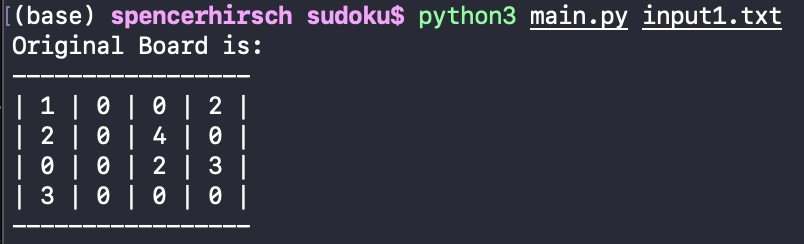
\includegraphics{compilation.png}

\textit{Screenshot demonstrating that the code runs.}

\pagebreak

\textbf{Screenshot showing output for first test case:}

\bigskip

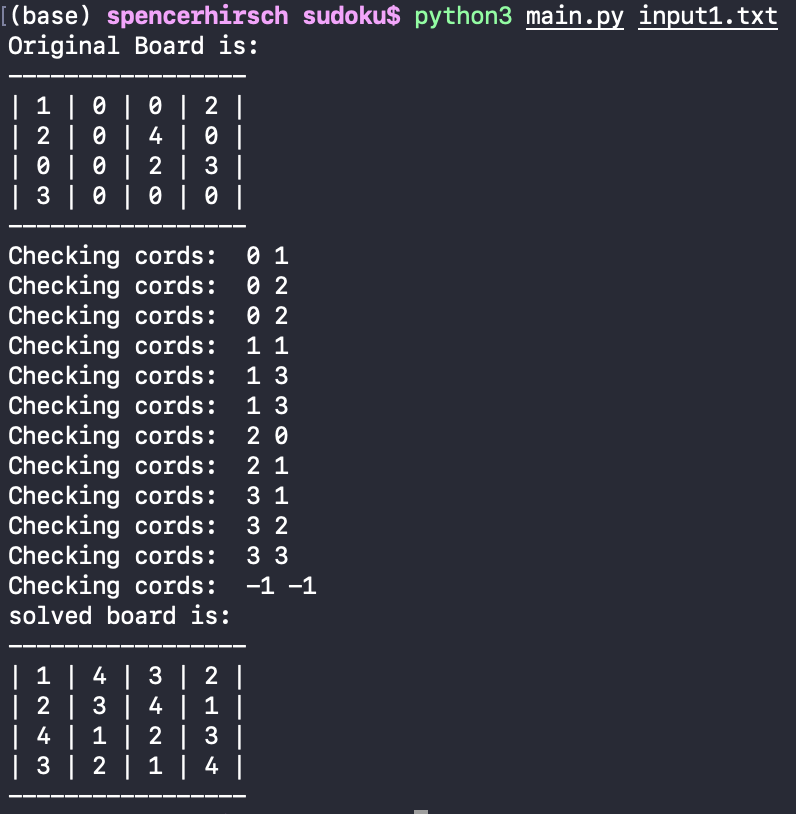
\includegraphics{test1.png}

\textit{Screenshot demonstrating our first test case, as well as correct output.}

\pagebreak

\textbf{Screenshot showing output for second test case:}

\bigskip

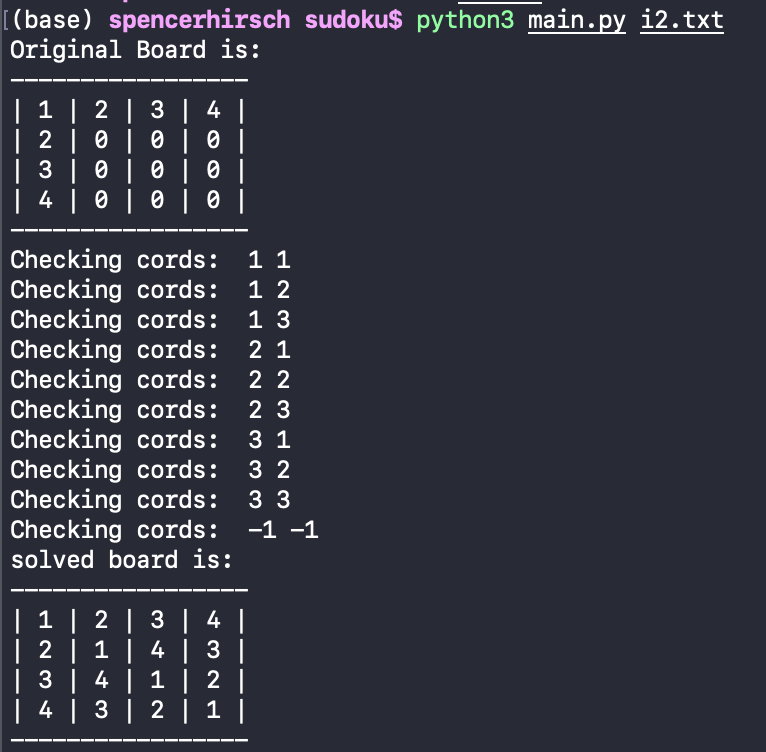
\includegraphics{test2.png}

\textit{Screenshot demonstrating our second test case, as well as the correct output.}

\pagebreak

\textbf{Screenshot showing output for third test case (impossible):}

\bigskip

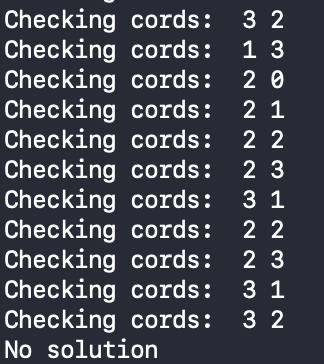
\includegraphics{impossible_output.png}

\textit{Screenshot demonstrating the output for an impossible puzzle given to the program.}

\pagebreak

\textbf{Screenshot showing output for fourth test case:}

\bigskip

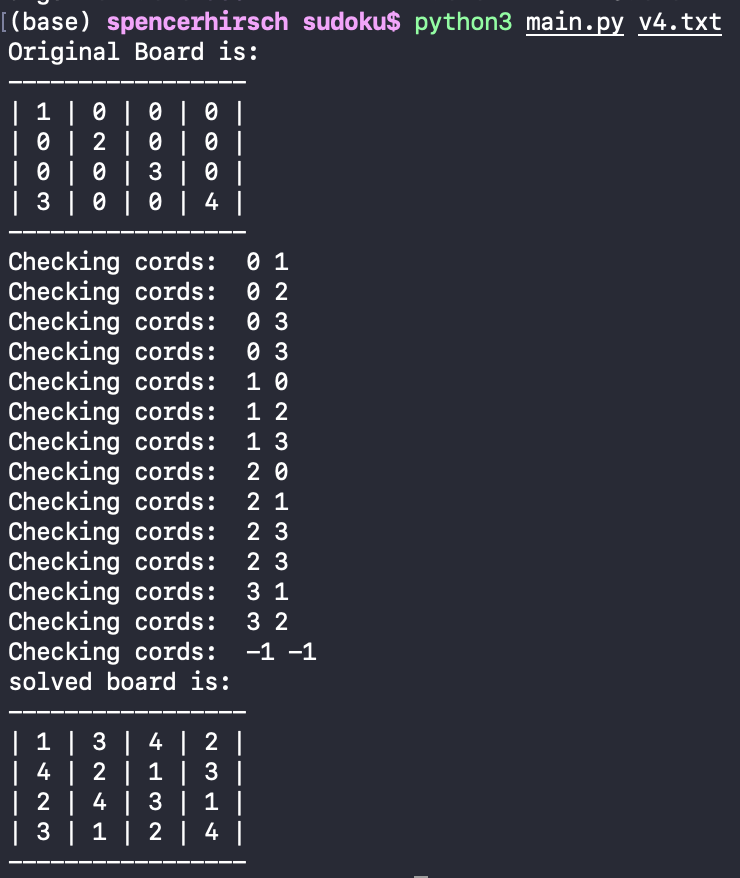
\includegraphics{test4.png}

\textit{Screenshot demonstrating the output for a fourth test case, for good measure.}

\pagebreak

\textbf{Summary of the intermediate submission:}

\bigskip

\noindent For this assignment, my partner and I used the backtracking algorithm in order
to solve for the problem. Our program reads in a text file that conatins the 
number of rows and columns as well as a list of the values that the matrix will
be made up of. The values will be read in by row,

\[R_{00},R_{01},R_{02},R_{03},R_{10},R_{11},R_{12},R_{13},R_{20},R_{21},R_{22},R_{23},R_{30},R_{31},R_{32},R_{33}\]

\noindent The values are then placed in their repsective places in the n $\times$ n matrix.
The initial empty spaces hold a value of 0, the algorithm will search for the 0's 
in the matrix and replace them with their correct value. We chose to use a backtracking
algorithm in order to solve this problem. The psuedo-code for our solution is posted above.
The solution that we came to is our original code.

\end{document}